\documentclass[../report.tex]{subfiles}
\begin{document}

\chapter{SimpLanPlus.java}\label{c:simplanplus-java}

\section{Che file è e a cosa serve}\label{s:che-file-cosa-serve}
Il file \textit{SimpLanPlus.java} contiene la definizione della classe Java \verb|SimpLanPlus| con al suo interno il metodo \verb|main|, ovvero il punto di partenza del compilatore ed interprete per \textbf{SimpLanPlus}.
È un file fondamentale: contiene tutti gli step che devono susseguirsi affinché entrambi i processi vadano a buon fine.
Si occupa:
\begin{itemize}
    \item di gestire i \textit{flag} passati assieme al lancio del programma;
    \item di leggere il contenuto dai file contenenti il codice sorgente;
    \item di gestire le eccezioni che possono verificarsi nel corso dell'esecuzione.
\end{itemize}

\section{Argomenti e flag}\label{s:argomenti-flag}
Oltre a quanto specificato al \hyperref[a:pt4]{punto 4} di \hyperref[a:installazione]{Guida all'installazione}, è possibile rendere flessibile il funzionamento del compilatore e dell'interprete.\\
C'è un unico argomento obbligatorio per avviare il programma, che è il nome del file da compilare e poi eseguire (che è come indicato al sopracitato punto 4). Se esso non viene specificato, viene visualizzato un errore:
\begin{figure}[H]
    \centering
    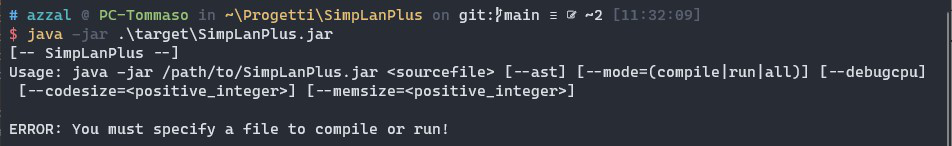
\includegraphics[width=0.98\textwidth]{argomentoNomeFileMancante}
    \caption{Avviso di mancanza del nome del file.}
    \label{fig:argomento-nome-file-mancante}
\end{figure}
\noindent
Se viene inserito il nome del file, allora il programma si avvia correttamente.\\
I \textit{flag} disponibili sono i seguenti:
\begin{itemize}
    \item \verb|--ast|, che permette di visualizzare, prima dell'esecuzione del codice \textbf{SVM-Assembly} generato, una versione testuale e \textit{human-readable} dell'AST (se non viene specificato, non viene mostrato);
    \item \verb/--mode=(compile|run|all)/, che permette di scegliere la modalità di avvio del programma:
    \begin{itemize}
        \item[*] \verb|compile| prende in input il file con codice sorgente \textbf{SimpLanPlus} specificato come primo argomento e restituisce in output un file con lo stesso nome, ma con estensione \textbf{.asm}, contenente il codice \textbf{SVM-Assembly} generato;
        \item[*] \verb|run| prende in input un file generato precedentemente (avviando il programma con il \textit{flag} \verb|--mode=compile|) e specificato come primo argomento al fine di eseguirlo;
        \item[*] \verb|all| prende in input il file con codice sorgente \textbf{SimpLanPlus} specificato come primo argomento, prima compilandolo, poi eseguendolo, senza generare file \textbf{.asm} intermedi;
    \end{itemize}
    Se non viene specificato, la modalità di avvio di default è \verb|--mode=all|;
    \item \verb|--debugcpu|, che permette graficamente di visualizzare lo stato della memoria e dei registri ad ogni istruzione del codice \textbf{SVM-Assembly} generato dal compilatore (se non viene specificato, non viene mostrato nulla). Il consiglio è di usare questo \textit{flag} assieme a un basso valore impostato su \verb|--memsize| (per piccoli programmi, empiricamente si è visto che 20 è spesso un buon valore);
    \item \verb|--codesize=<positive_integer>|, che permette di impostare il numero massimo di istruzioni macchina per cui c'è spazio nella ``memoria virtuale" in cui viene eseguito il codice \textbf{SVM-Assembly} generato (se non viene specificato o viene inserito un numero negativo, è 1000);
    \item \verb|--memsize=<positive_integer>|, che permette di impostare il numero massimo di celle di memoria per cui c'è spazio nella ``memoria virtuale" in cui viene eseguito il codice \textbf{SVM-Assembly} generato (se non viene specificato o viene inserito un numero negativo, è 1000);
\end{itemize}

\section{Compilazione}\label{s:compilazione}
La compilazione è gestita da \verb|String compile(final Flags flags, final String simpLanPlusCode)|, il metodo che esegue in ordine tutti gli step indicati brevemente in \hyperref[ss:compilatore]{Sezione 1.1.2 Il compilatore} e, più in dettaglio, nei \hyperref[c:analisi-semantica]{Capitolo 3 Analisi semantica}, \hyperref[c:analisi-effetti]{Capitolo 4 Analisi degli effetti}, \hyperref[c:typechecking]{Capitolo 5 Type checking}.
Il valore ritornato è la stringa contenente il codice \textbf{SVM-Assembly} generato a partire da quello \textbf{SimpLanPlus}.

\section{Esecuzione}\label{s:esecuzione}
L'esecuzione è gestita da \verb|void run(final Flags flags, final String assemblyCode)|, il metodo che esegue il codice \textbf{SVM-Assembly} passato come argomento in \verb|assemblyCode|, così come spiegato in maniera dettagliata in \hyperref[c:interprete]{Capitolo 6 Interprete}.


\end{document}

